% GENERATED FROM typst/manual/sections/01_rest_energy_prediction.typ BY scripts/typ2tex.py (v1.0.0) — DO NOT EDIT.
% Edit canonical Typst under typst/ and regenerate with: python3 scripts/typ2tex.py --root . --outdir latex

\section{Field Rest-Energy Records}\label{manual:rest-energy-prediction}

\paragraph{Setup and calculation card.}
Exact support/window declarations and zero-float \texttt{TritWord}/\texttt{TritRatio}
SADAR evaluations (vectors \texttt{RC-027}, \texttt{RC-028}, \texttt{RC-029}, and
\texttt{RC-011}) produce the A$\Omega$ accessor, collision-shedding debris, and internal
Higgs-selection records; measured masses remain quarantined external targets at
$B_{\mathrm{ext}}=\mathsf{Q}_{\mathrm{ext}}$ (\texttt{SD-007}, \texttt{SD-004},
\texttt{SD-005}) with the quoted uncertainties. A general rest-energy prediction still
requires this application's shared-history producer, history-to-rate map, relational
reference clock, and calibrated energy map. The Higgs table evaluates a separate
declared candidate/map diagnostic; its target-only pulls exclude model uncertainty.
Common comparison and source roles follow \secref{manual:calculation-spine}.

\subsection{0\texorpdfstring{$|-$}{|-} scope}\label{manual:rest:scope}

\paragraph{Setup.}
Rest-energy records separate exact internal A$\Omega$ field-map records (support,
carried cycle, and accessor values) from quarantined measured-sector target rows:

\[
\mathbf{a}\vdash(F,R,\partial_TR,\omega),\qquad B=(\partial_TF,\omega).
\]

The calculation spine is

\[
C_f[M]_{\AO}\longrightarrow\mathsf{AO}_{\mu}(C)\longrightarrow\SADARop_B(C)\longrightarrow\nu_{x,\AO}\longrightarrow E_{x,\mathrm{ext}}.
\]

\aodnoteblock{Data-support class}{Rest-energy records are D0 exact internal A$\Omega$ field records or O0 external-map comparisons, depending on the declared measured-sector target rows. Target uncertainties are supplied; input, reduction, and value-map contributions remain unresolved where no justified model is supplied.}

\aodprovenance{\mainappendix{main:app:ao-field-fractal-properties}.}

\subsection{Support notation used by the calculation records}\label{manual:rest:support-notation}

The manual uses compact support notation only where the calculation needs it:

\[
D_i\square D_j=\text{open-seat duon support},
\]

\[
D_i\mu D_j,\qquad\mu\in\{-1,0,+1\},\qquad=\text{resolved duon support},
\]

\[
E_2^0=\text{open-seat duon support},\qquad E_2^{\pm}=\text{duad / seated duon support}.
\]

The compact field supports are

\[
1:2:L=\text{Dimonon support},\qquad3:q:L=\text{Trion support}.
\]

Odd lengths are carried as odd-window route status between adjacent even support enclosures:

\[
L=2k+1\quad\Rightarrow\quad C_{2k}\leadsto L\leadsto C_{2k+2}.
\]

When this odd-window instability is retained as a route-status suffix, write $K_{\mathrm{yro}}$. Support-enclosure names remain the even-enclosure names.

\aodprovenance{\mainappendix{main:app:ao-field-fractal-properties}.}

\paragraph{Proposed supports and enclosure notation.}
Examples of proposed specifications are

\[
1:2:6=\text{Dimonhexon}=\text{Dimonon curling-curl support form carried on }C_6,
\]

and

\[
3:3:6=\text{Tritriohexon},\qquad3:4:6=\text{Tetratriohexon},
\]

on $C_6$. SADAR couples their retained beats after admission.

The shared hexon of \mainappendix{main:app:cc-basic-shared-hexon} expands as

\[
(3:3)^1::(3:4)^1::(1:2)^0::6.
\]

The separator rule in \mainsection{main:subsec:fractal-tesseract-cycle-range}
gives the following support parse:

\begin{equation}\label{eq:double-colon-parse-example}
3:4::3:3::6\equiv(3:4,3:3;C_6).
\end{equation}

\begin{table}[H]
\centering
\caption{Filled shared enclosure forms.}
\label{tab:cc-filled-shared-enclosures}
{\small
\begin{tabular}{lll}
\toprule
Compact form & Name & Outer enclosure \\
\midrule
$3:3:0::6$ & $\mathrm{Tritrio}^3::\mathrm{Tetratrio}^3::\mathrm{hexon}$ & hexon \\
$4:4:0::8$ & $\mathrm{Tritrio}^4::\mathrm{Tetratrio}^4::\mathrm{octon}$ & octon \\
$5:5:0::10$ & $\mathrm{Tritrio}^5::\mathrm{Tetratrio}^5::\mathrm{decon}$ & decon \\
\bottomrule
\end{tabular}
}
\end{table}

\subsubsection{Shared shell-path declaration}\label{subsec:shared-shell-path-declaration}

The shared shell-path declaration may be written

\[
0\mid-::Z:A:0:6\langle1:1:0::6\rangle.
\]

Named:

\[
0\mid-::Z:A:0:\mathrm{hexon}\langle\mathrm{Tritrio}::\mathrm{Tetratrio}::\mathrm{hexon}\rangle.
\]

For the filled hexon field, write

\[
0\mid-::Z:A:0:6\langle3:3:0::6\rangle.
\]

Named:

\[
0\mid-::Z:A:0:\mathrm{hexon}\langle\mathrm{Tritrio}^3::\mathrm{Tetratrio}^3::\mathrm{hexon}\rangle.
\]

\subsubsection{Nested shell-stack pattern}\label{subsec:nested-shell-stack-pattern}

The same curling-curl pattern iterates upward through shared enclosures and filled enclosures:

\[
\mathrm{Tritrio}^3::\mathrm{Tetratrio}^3::\mathrm{hexon}\to\mathrm{Tritrio}^4::\mathrm{Tetratrio}^4::\mathrm{octon}\to\mathrm{Tritrio}^5::\mathrm{Tetratrio}^5::\mathrm{decon}.
\]

\subsection{Field-property accessor calculations}\label{app:ao-field-fractal-properties:accessors-table}

Under the single-hinge neutral-reflection hypotheses of
\mainappendix{main:app:ao-field-fractal-properties:accessor}, the following
compatible native count windows give these nine accessor rows.
In the declared free-seat fixtures, $1:2\Rightarrow s=2$ and
$H_{\mu}^{[2]}=1$, while $3:3\Rightarrow s=1$ and
$H_{\mu}^{[1]}=1$. A full-seated single-hinge cycle uses
$H_{\mu}=H_{\mu}^{\mathrm{cyc}}=1$ unless free-seat provenance is declared.

\begin{table}[H]
\centering
\caption{A$\Omega$ field fractal properties.}
\label{tab:ao-field-fractal-properties}
{\footnotesize
\begin{tabular}{cllclcccccc}
\toprule
$\mathcal{F}_{\AO}$ & $M$ & $C_f[M]_{\AO}$ & $\Pi_{\alpha}$ & $H_{\mu}$ & $RD_{\AO}$ & $|\omega|$ & $\rho^D_{\omega}$ & $P^D$ & $Q^D$ & $X_{\mathrm{shedding}}$ \\
\midrule
$\mathfrak{f}_{1:2:6}$ & $1:2:6$ & $C_f[1:2]_{\AO}$ & 4 & $H_{\mu}^{[2]}=1$ & 9 & 6 & 6 & 18 & 9 & 0 \\
$\mathfrak{f}_{1:2:8}$ & $1:2:8$ & $C_f[1:2]_{\AO}$ & 4 & $H_{\mu}^{[2]}=1$ & 9 & 8 & 8 & 24 & 3 & 0 \\
$\mathfrak{f}_{1:2:9}$ & $1:2:9$ & $C_f[1:2]_{\AO}$ & 4 & $H_{\mu}^{[2]}=1$ & 9 & 9 & 9 & 27 & 0 & 3 \\
$\mathfrak{f}_{1:2:10}$ & $1:2:10$ & $C_f[1:2]_{\AO}$ & 4 & $H_{\mu}^{[2]}=1$ & 9 & 10 & 9 & 27 & 0 & 0 \\
$\mathfrak{f}_{3:2:6}$ & $3:2:6$ & $C_f[3:2]_{\AO}$ & 10 & 1 & 21 & 6 & 6 & 30 & 75 & 0 \\
$\mathfrak{f}_{3:2:8}$ & $3:2:8$ & $C_f[3:2]_{\AO}$ & 10 & 1 & 21 & 8 & 8 & 40 & 65 & 0 \\
$\mathfrak{f}_{3:2:10}$ & $3:2:10$ & $C_f[3:2]_{\AO}$ & 10 & 1 & 21 & 10 & 10 & 50 & 55 & 0 \\
$\mathfrak{f}_{3:3:6}$ & $3:3:6$ & $C_f[3:3]_{\AO}$ & 30 & $H_{\mu}^{[1]}=1$ & 61 & 6 & 6 & 36 & 330 & 0 \\
$\mathfrak{f}_{3:4:6}$ & $3:4:6$ & $C_f[3:4]_{\AO}$ & 68 & $H_{\mu}^{\mathrm{cyc}}=1$ & 137 & 6 & 6 & 42 & 917 & 0 \\
\bottomrule
\end{tabular}
}
\end{table}

For $3:4$, the single-hinge reduction of
\mainappendix{main:app:rd-tests:corollaries} gives

\begin{equation}\label{app:rd:eq:three-four-rd}
\Pi(3:4)=4^3+4=68,\qquad RD(3:4)=2\cdot68+1=137.
\end{equation}

The added $4$ is retained edge-shell support; the cycle object remains distinct from
this scalar accessor.

\paragraph{Derivation: support-multiplicity atlas and common span (\texttt{RC-029}).}
In \tabref{tab:ao-field-fractal-properties}, support-multiplicity pressure uses
$C_{\mathrm{sup}}(p:q)=p+q\in\{3,5,6,7\}$, giving
$P^D_{\mathrm{sup}}=(p+q)\rho^D_{\omega}$ and
$Q^D_{\mathrm{sup}}=(p+q)\max(0,RD-|\omega|)$, whereas
single-channel collision-pocket audits use scoped ternary continuation capacity
$C_3=3$ ($P^D_{\mathrm{chan}}=3\rho^D_{\omega}$). Verified in exact zero-float
arithmetic by vector \texttt{RC-029} (\texttt{sadar\_rest\_energy\_atlas},
\texttt{rest\_energy\_sadar\_debris\_atlas.csv}), the eight non-null recurring support
half-cycle step periods $2\Pi\in\{2,4,6,8,20,60,136\}$ (with $1:1$
doubled to $8$) fix the common four-phase bit-window span

\[
L_{\mathrm{common}}=4\cdot\operatorname{lcm}(2,4,6,8,20,60,136)=8160,
\]

strictly distinct from the summed eight-lineage closure tally
$0+60+136+408+1020+1360+2040+4080=9104$ over that common span, while
preserving exact native reflection-duration ratios
$RD(3:3)/RD(1:2)=61/9$,
$RD(3:4)/RD(3:3)=137/61$, and
$RD(3:2)/RD(1:2)=21/9=7/3$.

\begin{figure}[H]
\centering
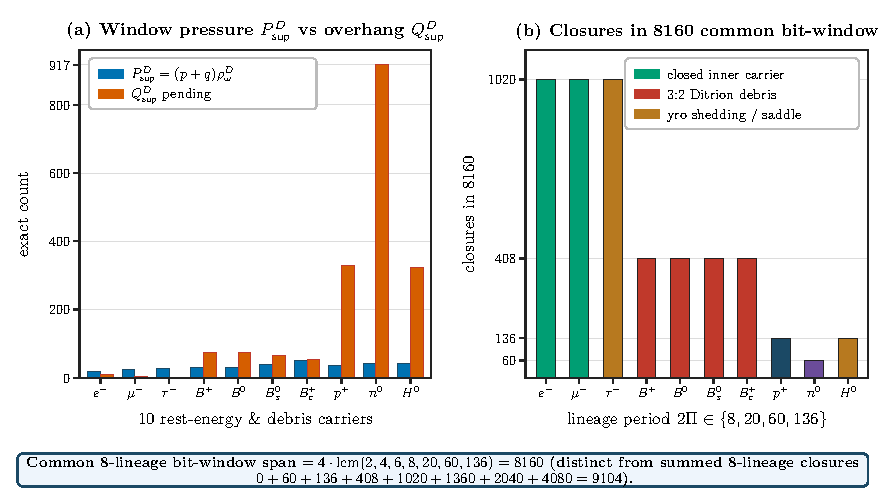
\includegraphics[width=0.92\linewidth,height=0.78\textheight,keepaspectratio]{figures/generated/rest-energy-stability-debris-atlas.pdf}
\caption{Exact support window pressure $P^D_{\mathrm{sup}}$, pending overhang $Q^D_{\mathrm{sup}}$, and closure counts per $8160$ common bit-window span across all ten rest-energy and collision-shedding debris carriers (\texttt{RC-029}, \texttt{rest\_energy\_sadar\_debris\_atlas.csv}).}
\label{fig:manual-rest-energy-debris-atlas}
\end{figure}

\subsection{A\texorpdfstring{$\Omega$}{Omega} field-map table}\label{manual:rest:ao-field-value-table}

The A$\Omega$ field-map table lists the manual mapping from measured-sector names to A$\Omega$ field supports. The numerical field-support properties are calculated in
\tabref{tab:ao-field-fractal-properties}.

\begin{table}[H]
\centering
\caption{A$\Omega$ field-map table.}
\label{tab:manual-ao-field-value-table}
{\footnotesize
\begin{tabular}{lllll}
\toprule
$x_{\mathrm{ext}}$ & external map & $M_x$ & $C_f[M_x]_{\AO}$ & $\nu_{x,\AO}$ \\
\midrule
$e^-$ & $00|-$ Dimonhexon & $1:2:6$ & $C_f[1:2]_{\AO}$ & $\nu_{e,\AO}$ \\
$\mu^-$ & $00|-$ Dimonocton & $1:2:8$ & $C_f[1:2]_{\AO}$ & $\nu_{\mu,\AO}$ \\
$\tau^-$ & $00|-$ Dimonnanyro & $1:2:9_{\mathrm{yro}}$ & $C_f[1:2]_{\AO}$ & $\nu_{\tau,\AO}$ \\
$B^{\pm}$ & Ditrion debris map & $3:2:6$ & $C_f[3:2]_{\AO}$ & $\nu_{B,\AO}$ \\
$B^0$ & Ditrion debris map & $3:2:6$ & $C_f[3:2]_{\AO}$ & $\nu_{B,\AO}$ \\
$B_s^0$ & lifted Ditrion map & $3:2:8$ & $C_f[3:2]_{\AO}$ & $\nu_{B_s,\AO}$ \\
$B_c^{\pm}$ & lifted Ditrion map & $3:2:10$ & $C_f[3:2]_{\AO}$ & $\nu_{B_c,\AO}$ \\
$p^+$ & Tritriohexon map & $3:3:6$ & $C_f[3:3]_{\AO}$ & $\nu_{p,\AO}$ \\
$n^0$ & Tetratriohexon map & $3:4:6$ & $C_f[3:4]_{\AO}$ & $\nu_{n,\AO}$ \\
\bottomrule
\end{tabular}
}
\end{table}

\aodprovenance{\mainappendix{main:app:ao-field-fractal-properties}; \mainsection{main:subsec:curling-curl-support-forms}.}

\aodremark{The manual declares measured-sector maps such as $e^-\mapsto00|-$ Dimonhexon. These maps are carried by manual comparison records; \tabref{tab:ao-field-fractal-properties} lists the A$\Omega$ field-property calculations.}

\paragraph{Falsification: support degeneracy and held-out discipline.}
The displayed $B^{\pm}$ and $B^0$ rows share the same retained support $3:2:6$.
Any mass map using support scalar $RD=21$ alone cannot distinguish those two targets;
a rest-energy application must bind additional shell-seat state with a matched
nondegeneracy witness (supplied below via \texttt{RC-028}) or declare limited resolution.
A target is held out only when its exclusion from construction, selection, and
calibration is explicitly bound.

\subsection{Boundary-full SADAR rest-energy closures and collision-shedding debris}\label{manual:rest:boundary-sadar-debris}

\paragraph{Setup and engine verification.}
All ten rest-energy and collision-shedding debris carriers in
\tabref{tab:manual-ao-field-value-table} and
\secref{manual:tritrioseptyro-higgs-support-fixture} execute in pure zero-float
\texttt{TritWord}/\texttt{TritRatio} arithmetic without hardcoded winners or asserted
slot literals via the \texttt{boundary\_sadar} sector
(\texttt{python3 -B -m manual.engine --sector boundary\_sadar} and
\texttt{aod-core --verify-vectors --check-zero-float}) across vectors \texttt{RC-027}
(\texttt{sadar\_pp\_tau\_five\_boundary}), \texttt{RC-028}
(\texttt{sadar\_hadron\_debris\_and\_higgs\_saddle}), \texttt{RC-029}
(\texttt{sadar\_rest\_energy\_atlas}), and quarantined external target-rate verification
\texttt{SD-007} (\texttt{sadar\_rest\_energy\_qext}). Their topological regimes partition
into four boundary classes (Figure~\ref{fig:manual-collision-debris-feynman}):

1. \textbf{Seated inner even closures ($X_{\mathrm{shedding}}=0$, \texttt{RC-029}):} On even support enclosures $\mathsf{C}_6$ and $\mathsf{C}_8$, Dimonhexon ($e^-$, $1:2:6$, $RD=9$), Dimonocton ($\mu^-$, $1:2:8$, $RD=9$), Tritriohexon ($p^+$, $3:3:6$, $RD=61$), and Tetratriohexon ($n^0$, $3:4:6$, $RD=137$) close internally without shedding surplus, preserving exact native reflection-duration ratios $RD(3:3)/RD(1:2)=61/9$ and $RD(3:4)/RD(3:3)=137/61$.

2. \textbf{Five-boundary SADAR collision-shedding stack for Tau ($1:2:9_{\mathrm{yro}}$ Dimonnanyro, \texttt{RC-027}):} Declare the ordered boundary stack $B_{\mathrm{hard}}\to B_{\tau}\to B_{\mathrm{shed}}\to B_{\mathrm{sensor}}\to B_{\mathrm{ext}}$ (Figure~\ref{fig:manual-tau-five-boundary-sadar}, \tabref{tab:manual-tau-five-boundary-trace}).
\begin{itemize}
\item \textbf{Hard cavity ($B_{\mathrm{hard}}$):} Opposing \texttt{pp} $3:3:6+3:3:6$ baryon streams couple across \texttt{BETWEEN} $E_2$ duon chiral flips (\texttt{window\_duons = 3}, \texttt{lead\_lag = 8}), achieving early coupling at cut $1$ with exact raw cut accounting \texttt{raw\_cuts = 28 = 11 + 17}: live \texttt{TritWord.burn\_contiguous\_dwell(keep\_single\_dwell=False)} burns $17$ optional $0_D$ (\texttt{00}) dwell lanes while preserving structural $0_H$ (\texttt{11}) hinges, leaving $11$ symmetry-quotient cuts ($17$ chiral flips, total attention $24/5$, and moving-boundary Stokes tally $18-22+3=-1$). Removing \texttt{BETWEEN} duon coupling (\texttt{duons = 0}) yields the sterile negative control, remaining uncoupled through cut $58$ ($48$ H1 moves, $16$ structural $0_H$ hinges, zero chiral flips, $X_{\mathrm{shedding}}=0$).
   - \textbf{Lepton pocket competition ($B_{\tau}$):} Evaluating the full $1:2:L$ family ($RD=9$, $C_3=3$) across $L\in\{2,6,7,8,9,10\}$, even windows $1:2:2$, $1:2:6$, and $1:2:8$ close internally ($X_{\mathrm{shedding}}=0$); short odd window $1:2:7$ retains incomplete overhang $Q^D=6$ with $\mathsf{C}_8$ deficit $\Delta^{\mathrm{close}}=-3$; window $1:2:10$ clips at $\rho^D_{\omega}=\min(9,10)=9$ and closes on $\mathsf{C}_{10}=27$ ($X_{\mathrm{shedding}}=0$); and $1:2:9_{\mathrm{yro}}$ uniquely exhausts full Dimonon duration ($Q^D=0$) while exceeding $\mathsf{C}_8=24$ with positive shedding surplus $X_{\mathrm{shedding}}=27-24=3$.
   - \textbf{Derived $50$-microslot $Q_4\times\mu$ impedance rotor ($B_{\mathrm{shed}}\to B_{\mathrm{sensor}}$):} Instead of asserting slot literals, the deterministic $50$-microslot $Q_4\times\mu$ impedance rotor (4D capacity $4\times50=200$) steps across the native reflection-duration ladder $RD=9\to61\to137$. Stage 1 at $B_{\mathrm{shed}}$ ($1:2\to3:3$, $\Delta RD=61-9=52$) dynamically produces exact $(13/50,37/50)$ for inner endoshedding versus outward exoshedding (\texttt{\_Exo}). Stage 2 at the passive \texttt{ReadOnly} $3:4:6$ sensor wall $B_{\mathrm{sensor}}$ ($3:3\to3:4$, $\Delta RD=137-61=76$, zero observer back-reaction onto the cavity) dynamically produces conditional \texttt{\_Exo} fractions $(19/50,31/50)$ for visible seating versus unseated traversal (exact missing burden $\operatorname{miss}_{\tau}=31/50$). Their two-stage product gives exact $2500$-slot conservation $(650/2500,1850/2500)$ for endoshedding versus \texttt{\_Exo} and $(703/2500,1147/2500)$ for visible versus unseated traversal ($650+703+1147=2500$, conditional \texttt{\_Exo} ratios $703/1850=19/50$ and $1147/1850=31/50$) along the witness-ordered recipient lattice \texttt{emitted -> delivered -> accepted -> seated -> closed\_origin} ($\Delta\operatorname{bip}=0$) \texttt{-> reclosed} ($\Delta\operatorname{bip}=+1$). Quarantined target comparison enters only at $B_{\mathrm{ext}}=\mathsf{Q}_{\mathrm{ext}}$ (\texttt{SD-007}).
\end{itemize}
3. \textbf{Core-starvation $3:3\to3:2$ Ditrion collision-shedding debris ($RD=21$, \texttt{RC-028} and \texttt{RC-029}):} When a hard baryon collision pocket sheds one inner branch role from $3:3$ ($\Pi=30$, $RD=61$) into $3:2$ Ditrion support ($\Pi=2^3+2=10$, $RD=21$), the debris enters even enclosures as transient meson remnants (\texttt{rest\_energy\_sadar\_debris\_atlas.csv}, vectors \texttt{RC-028} and \texttt{RC-029}). On $3:2:6$, support scalar $RD=21$ alone is degenerate between $B^{\pm}$ and $B^0$; shell-dressing chirality in \texttt{ChiralPair4} resolves $B^{\pm}$ as seated duad $E_2^{\pm}$ ($\chi_{\mathrm{shell}}=\pm1$, structural $0_H$ present) and $B^0$ as open-seat duon $E_2^0$ ($\chi_{\mathrm{shell}}=0$, structural $0_H$ absent). Under higher collision-pocket pressure, exoshedding lifts the $3:2$ Ditrion core across adjacent even enclosures $3:2:6\to3:2:8$ ($B_s^0$, $P^D_{\mathrm{sup}}=40$, $Q^D_{\mathrm{sup}}=65$) $\to3:2:10$ ($B_c^{\pm}$, $P^D_{\mathrm{sup}}=50$, $Q^D_{\mathrm{sup}}=55$).

4. \textbf{Symmetric $\mathsf{C}_6/\mathsf{C}_8$ baryon-overlap saddle ($3:3:7_{\mathrm{yro}}$, \texttt{RC-028}):} Two-baryon $3:3+3:3$ overlap midpoint selection is audited in the Tritrioseptyro Higgs-support diagnostic below.

\begin{figure}[H]
\centering
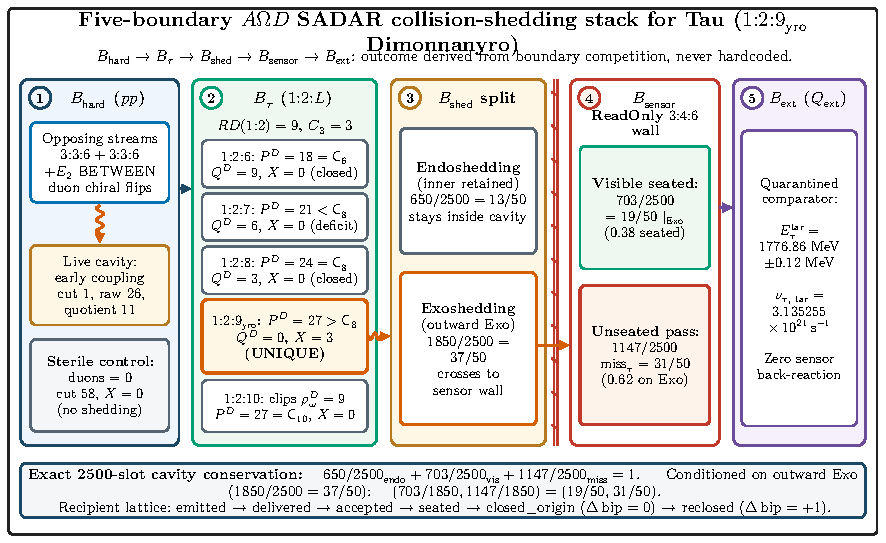
\includegraphics[width=0.92\linewidth,height=0.78\textheight,keepaspectratio]{figures/generated/tau-five-boundary-sadar-setup.pdf}
\caption{Five-boundary A$\Omega$D SADAR stack $B_{\mathrm{hard}}\to B_{\tau}\to B_{\mathrm{shed}}\to B_{\mathrm{sensor}}\to B_{\mathrm{ext}}$ for $1:2:9_{\mathrm{yro}}$ Dimonnanyro (\texttt{RC-027}, \texttt{tau\_five\_boundary\_sadar\_trace.csv}).}
\label{fig:manual-tau-five-boundary-sadar}
\end{figure}

\begin{figure}[H]
\centering
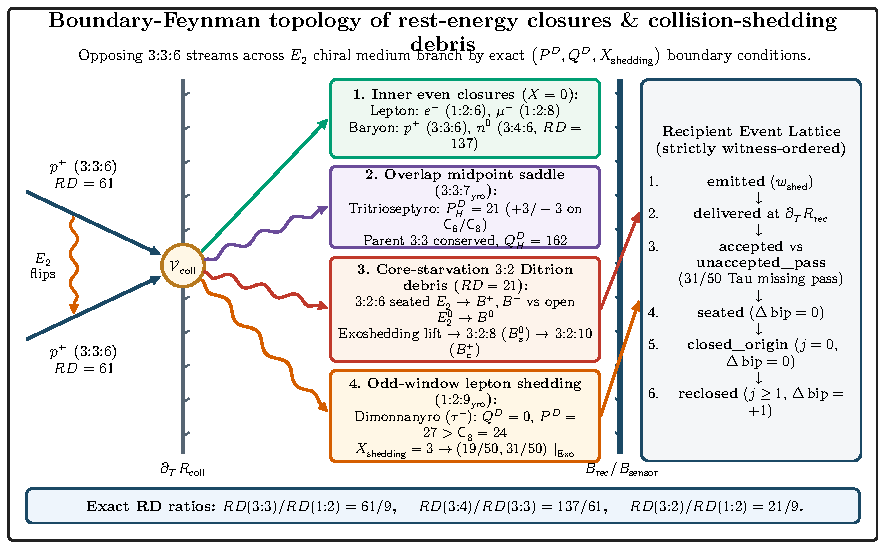
\includegraphics[width=0.92\linewidth,height=0.78\textheight,keepaspectratio]{figures/generated/collision-shedding-debris-feynman.pdf}
\caption{Boundary-Feynman branching of inner even closures (\texttt{RC-029}), $3:3:7_{\mathrm{yro}}$ overlap-saddle selection and $3:2$ Ditrion core-starvation debris (\texttt{RC-028}), and $1:2:9_{\mathrm{yro}}$ odd-window lepton shedding (\texttt{RC-027}) into the witness-ordered recipient event lattice.}
\label{fig:manual-collision-debris-feynman}
\end{figure}

\begin{table}[H]
\centering
\caption{Engine-bound five-boundary SADAR competition table (\texttt{RC-027}, live from \texttt{manual/data/boundary\_sadar/tau\_five\_boundary\_sadar\_trace.csv}).}
\label{tab:manual-tau-five-boundary-trace}
{\scriptsize
\begin{tabular}{>{\raggedright\arraybackslash}p{0.088\linewidth}>{\raggedleft\arraybackslash}p{0.050\linewidth}>{\raggedleft\arraybackslash}p{0.050\linewidth}>{\raggedleft\arraybackslash}p{0.050\linewidth}>{\raggedleft\arraybackslash}p{0.050\linewidth}>{\raggedleft\arraybackslash}p{0.050\linewidth}>{\raggedleft\arraybackslash}p{0.050\linewidth}>{\raggedleft\arraybackslash}p{0.092\linewidth}>{\raggedleft\arraybackslash}p{0.114\linewidth}>{\raggedright\arraybackslash}p{0.280\linewidth}}
\toprule
Candidate & $L$ & $\rho^D_{\omega}$ & $P^D$ & $Q^D$ & $C_{\mathrm{close}}$ & $X_{\mathrm{shed}}$ & Endo / Exo & Vis / Miss $|_{\mathrm{Exo}}$ & Boundary stack \& SADAR verdict \\
\midrule
\texttt{3:3:6+\allowbreak{}3:3:6\_\allowbreak{}duons0} & 58 & 0 & 0 & 0 & 0 & 0 & 0/1\par 0/1 & 0/1\par 0/1 & \texttt{B\_\allowbreak{}hard\_\allowbreak{}sterile\_\allowbreak{}control}\par \texttt{sterile\_\allowbreak{}cut58\_\allowbreak{}no\_\allowbreak{}BETWEEN\_\allowbreak{}coupling} \\
\texttt{1:2:2} & 2 & 2 & 6 & 21 & 6 & 0 & 1/1\par 0/1 & 0/1\par 0/1 & \texttt{B\_\allowbreak{}hard->\allowbreak{}B\_\allowbreak{}cand\_\allowbreak{}inner\_\allowbreak{}retained}\par \texttt{closed\_\allowbreak{}or\_\allowbreak{}clipped\_\allowbreak{}unseen\_\allowbreak{}at\_\allowbreak{}sensor\_\allowbreak{}wall} \\
\texttt{1:2:6} & 6 & 6 & 18 & 9 & 18 & 0 & 1/1\par 0/1 & 0/1\par 0/1 & \texttt{B\_\allowbreak{}hard->\allowbreak{}B\_\allowbreak{}cand\_\allowbreak{}inner\_\allowbreak{}retained}\par \texttt{closed\_\allowbreak{}or\_\allowbreak{}clipped\_\allowbreak{}unseen\_\allowbreak{}at\_\allowbreak{}sensor\_\allowbreak{}wall} \\
\texttt{1:2:7} & 7 & 7 & 21 & 6 & 24 & 0 & 1/1\par 0/1 & 0/1\par 0/1 & \texttt{B\_\allowbreak{}hard->\allowbreak{}B\_\allowbreak{}cand\_\allowbreak{}open\_\allowbreak{}deficit}\par \texttt{incomplete\_\allowbreak{}RD\_\allowbreak{}QD6\_\allowbreak{}c8\_\allowbreak{}deficit} \\
\texttt{1:2:8} & 8 & 8 & 24 & 3 & 24 & 0 & 1/1\par 0/1 & 0/1\par 0/1 & \texttt{B\_\allowbreak{}hard->\allowbreak{}B\_\allowbreak{}cand\_\allowbreak{}inner\_\allowbreak{}retained}\par \texttt{closed\_\allowbreak{}or\_\allowbreak{}clipped\_\allowbreak{}unseen\_\allowbreak{}at\_\allowbreak{}sensor\_\allowbreak{}wall} \\
\texttt{1:2:9} & 9 & 9 & 27 & 0 & 24 & 3 & 650/2500\par 1850/2500 & 19/50\par 31/50 & \texttt{B\_\allowbreak{}hard->\allowbreak{}B\_\allowbreak{}tau->\allowbreak{}B\_\allowbreak{}shed->\allowbreak{}B\_\allowbreak{}sensor->\allowbreak{}B\_\allowbreak{}ext}\par \texttt{unique\_\allowbreak{}QD0\_\allowbreak{}shedder\_\allowbreak{}Dimonnanyro\_\allowbreak{}winner} \\
\texttt{1:2:10} & 10 & 9 & 27 & 0 & 27 & 0 & 1/1\par 0/1 & 0/1\par 0/1 & \texttt{B\_\allowbreak{}hard->\allowbreak{}B\_\allowbreak{}cand\_\allowbreak{}inner\_\allowbreak{}retained}\par \texttt{closed\_\allowbreak{}or\_\allowbreak{}clipped\_\allowbreak{}unseen\_\allowbreak{}at\_\allowbreak{}sensor\_\allowbreak{}wall} \\
\bottomrule
\end{tabular}
}
\end{table}

\subsection{Electron external map}\label{manual:rest:electron-external-map}

\paragraph{Specialization.}
The electron comparison record is a manual map from the measured-sector electron to the A$\Omega$ Dimonhexon support:

\[
e^-\longmapsto00|-\;\mathrm{Dimonhexon}\equiv00|-\;(1:2:6),\qquad C_f[1:2]_{\AO}.
\]

The charge-orientation tag is

\[
q_{\mathrm{ext}}(e^-)=-1,\qquad Q_{\mathrm{ext}}(e^-)=-e.
\]

The rest-energy comparison target remains quarantined at $B_{\mathrm{ext}}=\mathsf{Q}_{\mathrm{ext}}$ (\texttt{SD-007}):

\[
E^{\mathrm{tar}}_e=0.51099895069\,\mathrm{MeV},\qquad\sigma_{E,e}=1.6\times10^{-10}\,\mathrm{MeV}.
\]

\aodliteraturenote{Electron mass-energy: NIST CODATA~\cite{nist-electron-mass-energy}, SI defining constants: BIPM~\cite{bipm-si-defining-constants}.}

\aodremark{The $00|-$ tag is a manual measured-sector charge/orientation map carried by the manual comparison record.}

\subsection{Measured rest-energy target records}\label{manual:rest:measured-comparison-analysis}

\paragraph{Quarantined external comparison (\texttt{SD-007}).}
External comparison enters strictly at $B_{\mathrm{ext}}=\mathsf{Q}_{\mathrm{ext}}$.
For records with declared targets,

\[
E_{x,\mathrm{ext}}=K_{\mathrm{ext}}\nu_{x,\AO},\qquad\Delta E_x=E_{x,\mathrm{ext}}-E_x^{\mathrm{tar}},
\]

\[
\epsilon_x^{\mathrm{sgn}}=100\frac{\Delta E_x}{E_x^{\mathrm{tar}}},\qquad|\epsilon_x|=|\epsilon_x^{\mathrm{sgn}}|,\qquad z_{x,\mathrm{target}}=\frac{\Delta E_x}{\sigma_{E,x}}.
\]

Vector \texttt{SD-007} (\texttt{sadar\_rest\_energy\_qext}) verifies exact BIPM 2019 SI
rational $K_{\mathrm{ext}}$ target-rate inversion and zero round-trip
$\eta_{\mathrm{ext}}$ residual across all nine measured target rows below (tabulated
alongside native invariants in \texttt{rest\_energy\_sadar\_debris\_atlas.csv}).

\begin{table}[H]
\centering
\caption{Measured rest-energy target records (quarantined $B_{\mathrm{ext}}$ audit in \texttt{SD-007}).}
\label{tab:manual-measured-comparison-analysis}
{\footnotesize
\begin{tabular}{lrrll}
\toprule
Record & Target [MeV] & $\sigma_E$ [MeV] & Unit & Source \\
\midrule
$e$ & $0.51099895069$ & $1.6\times10^{-10}$ & MeV & NIST CODATA \\
$\mu$ & $105.6583755$ & $2.3\times10^{-6}$ & MeV & NIST CODATA \\
$\tau$ & $1776.86$ & $0.12$ & MeV & NIST / PDG target record \\
$B^{\pm}$ & $5279.41$ & $0.07$ & MeV & PDG 2025 \\
$B^0$ & $5279.72$ & $0.08$ & MeV & PDG 2025 \\
$B_s^0$ & $5366.93$ & $0.10$ & MeV & PDG 2025 \\
$B_c^{\pm}$ & $6274.47$ & $0.32$ & MeV & PDG 2025 \\
$p$ & $938.27208943$ & $2.9\times10^{-7}$ & MeV & NIST CODATA \\
$n$ & $939.56542194$ & $4.8\times10^{-7}$ & MeV & NIST CODATA \\
\bottomrule
\end{tabular}
}
\end{table}

\aodprovenance{\mainappendix{main:app:ao-field-fractal-properties};
\appref{manual:external-comparison}.}

\aodliteraturenote{Lepton/baryon targets: NIST CODATA~\cite{nist-electron-mass-energy,nist-muon-mass-energy,nist-tau-mass-energy,nist-proton-mass-energy,nist-neutron-mass-energy}, meson targets: PDG 2025~\cite{pdg-bmeson-2025}.}

\subsection{Tritrioseptyro Higgs-support diagnostic fixture}\label{manual:tritrioseptyro-higgs-support-fixture}

\paragraph{Setup and falsification boundary.}
The supplied candidate rows and scoring formula reproduce the internal ranking; they do
not supply the originating history producer, detector thresholds, or exposure history of
the scale/exponent choice. Recovering those artifacts remains this application's next
step before an independent prediction claim, and the freeze order below states the
declared evaluation order rather than a historical pre-exposure freeze.

Tritrioseptyro is the $3:3:7_{\mathrm{yro}}$ Higgs-support prediction candidate
selected by the internal AFC trace. The AFC run produces the read-only trace rows;
A$\Omega$ detectors read the trace and name the retained route status before joining to
the frozen external mass map $E_H=RD\,2^{L+4}$ MeV. Production-channel and
decay-channel residual tables carry the next comparison layer.

\[
\text{AFC run}\longrightarrow\text{read-only trace}\longrightarrow\text{A}\Omega\text{ route-status naming}.
\]

The trace is read-only for this record; feedback experiments require separately declared
write-back maps.

\paragraph{Derivation.}
Declare the odd-window trion candidate set

\[
\mathcal{K}_H=\{3:1:7,3:1:9,3:2:7,3:2:9,3:3:7,3:3:9,3:4:7,3:4:9\}.
\]

For each candidate $K=(p,q,L)$, compute

\[
\Pi=q^p+q,\qquad RD=2\Pi+1,\qquad\rho^D_{\omega}=\min(RD,L),
\]

with scoped collision capacity

\[
C_{3,H}=3,
\]

giving active window pressure and pending overhang

\begin{align*}
P^D_H & =C_{3,H}\rho^D_{\omega},\\Q^D_H & =C_{3,H}\max(0,RD-L).
\end{align*}

\paragraph{Specialization (\texttt{RC-011} and \texttt{RC-028}).}
The retained candidate is

\[
K_H^{\star}=3:3:7_{\mathrm{yro}}=\mathrm{Tritrioseptyro}.
\]

For Tritrioseptyro,

\[
\Pi=30,\qquad RD=61,\qquad\rho^D_{\omega}=7,\qquad P^D_H=21,\qquad Q^D_H=162,
\]

with symmetric residuals against adjacent even support-enclosure closures:

\[
P^D_H-C_6=+3,\qquad P^D_H-C_8=-3.
\]

The trace places Tritrioseptyro on the $C_6/C_8$ saddle with pressure residuals $+3$ and $-3$ and pending overhang $Q^D_H=162$.

\begin{table}[H]
\centering
\caption{Higgs-support candidate ranking. This table carries the active trace coordinates used by the internal selection rule (\texttt{RC-011}).}
\label{tab:manual-higgs-internal-candidates}
{\footnotesize
\begin{tabular}{lrrrrr}
\toprule
Candidate & $RD$ & $P^D_H$ & saddle & $Q^D_H$ & score \\
\midrule
$3:3:7_{\mathrm{yro}}$ & $61$ & $21$ & $+3/-3$ & $162$ & $0.00$ \\
$3:2:7_{\mathrm{yro}}$ & $21$ & $21$ & $+3/-3$ & $42$ & $1.58$ \\
$3:3:9_{\mathrm{yro}}$ & $61$ & $27$ & $+3/0$ & $156$ & $2.25$ \\
$3:4:7_{\mathrm{yro}}$ & $137$ & $21$ & $+3/-3$ & $390$ & $2.40$ \\
$3:2:9_{\mathrm{yro}}$ & $21$ & $27$ & $+3/0$ & $36$ & $2.89$ \\
$3:1:7_{\mathrm{yro}}$ & $5$ & $15$ & $-3/-9$ & $0$ & $3.00$ \\
$3:4:9_{\mathrm{yro}}$ & $137$ & $27$ & $+3/0$ & $384$ & $3.59$ \\
$3:1:9_{\mathrm{yro}}$ & $5$ & $15$ & $-9/-12$ & $0$ & $4.75$ \\
\bottomrule
\end{tabular}
}
\end{table}

The trace score is verified in exact zero-float rational arithmetic by vector
\texttt{RC-011} (\texttt{higgs\_trace\_score\_and\_freeze}, yielding $S_H(3:3:7)=0$
versus runner-up $S_H(3:2:7)=79/50=1.58$) under the internal selection rule:

\[
S_H(K)=\frac{d_{\mathrm{saddle}}}{12}+\frac{d_Q}{100}+\frac{d_L}{2}+d_{\mathrm{route}},\qquad\arg\min_{K\in\mathcal{K}_H}S_H(K)=3:3:7_{\mathrm{yro}}.
\]

\aodnoteblock{Source artifacts}{The score-component definitions and candidate rows are supplied under \texttt{manual/data/higgs} as \texttt{higgs\_trace\_score\_formula.md} and \texttt{higgs\_trace\_internal\_candidates\_selection.csv}, respectively.}

Alongside the legacy ranking formula $S_H(K)$, vector \texttt{RC-028}
(\texttt{sadar\_hadron\_debris\_and\_higgs\_saddle},
\texttt{manual/data/boundary\_sadar/higgs\_baryon\_overlap\_saddle\_scan.csv}) evaluates the
full $20$-candidate trion grid $3:q:L$ ($q\in\{1,2,3,4\}$,
$L\in\{6,7,8,9,10\}$) without empirical overhang-band thresholds: exact
symmetric $\mathsf{C}_6/\mathsf{C}_8$ midpoint balance
$(P^D_H-\mathsf{C}_6)+(P^D_H-\mathsf{C}_8)=0$ ($P^D_H=21$) holds only on
$\{3:2:7,3:3:7,3:4:7\}$, and two-baryon $3:3+3:3$ parent
lineage conservation ($q=3$) isolates $3:3:7_{\mathrm{yro}}$ uniquely prior to
external map freeze.

\begin{figure}[H]
\centering
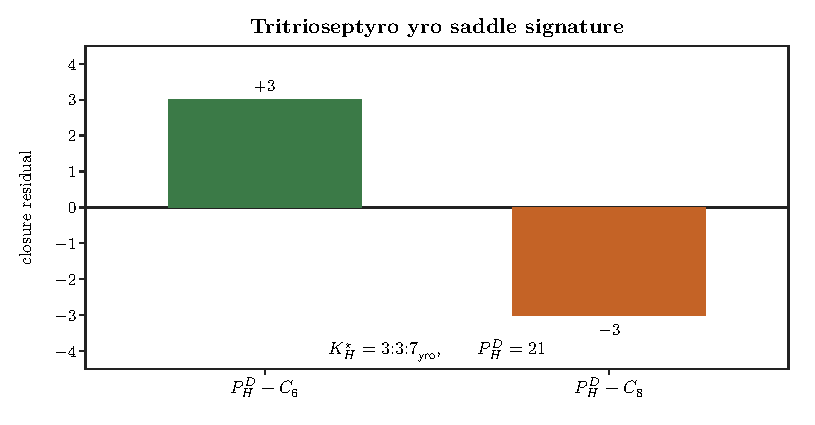
\includegraphics[width=0.92\linewidth,height=0.78\textheight,keepaspectratio]{figures/generated/higgs-yro-saddle-signature.pdf}
\caption{Tritrioseptyro yro saddle signature. The internal AFC trace gives $P^D_H=21$, placing the selected $3:3:7_{\mathrm{yro}}$ candidate between $C_6=18$ and $C_8=24$ with residuals $+3$ and $-3$.}
\label{fig:manual-higgs-yro-saddle}
\end{figure}

\begin{figure}[H]
\centering
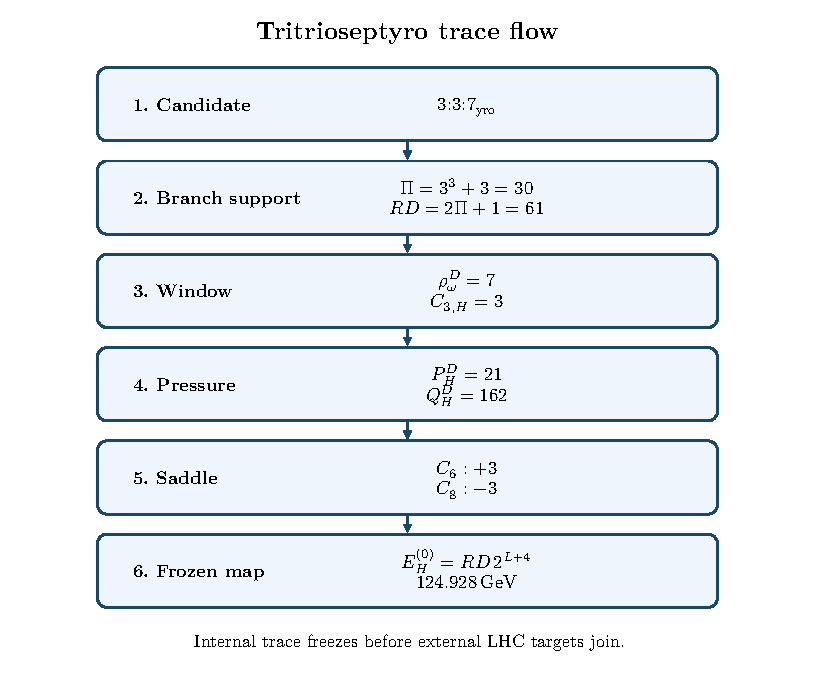
\includegraphics[width=0.92\linewidth,height=0.78\textheight,keepaspectratio]{figures/generated/higgs-tritrioseptyro-trace-flow.pdf}
\caption{Tritrioseptyro trace flow. The AFC run produces $\Pi=30$, $RD=61$, $\rho^D_{\omega}=7$, $P^D_H=21$, and $Q^D_H=162$. A$\Omega$ names the detected $3:3:7_{\mathrm{yro}}$ route status as Tritrioseptyro.}
\label{fig:manual-higgs-trace-flow}
\end{figure}

\subsubsection{External mass map after candidate freeze}\label{manual:higgs-external-map-after-freeze}

\paragraph{Specialization (\texttt{RC-011}, \texttt{SD-004}, \texttt{SD-005}).}
The external mass map is frozen strictly after the internal candidate is selected:

\[
E_H^{(0)}[\mathrm{MeV}]=RD_H\,2^{L+4}.
\]

For Tritrioseptyro (verified in exact rational arithmetic by \texttt{RC-011} as
$15616/125\,\mathrm{GeV}$),

\[
E_H^{(0)}=61\cdot2^{11}\,\mathrm{MeV}=124928\,\mathrm{MeV}=124.928\,\mathrm{GeV}.
\]

Declared LHC Higgs mass targets enter strictly after candidate and map freeze. Each
comparison row reports $\Delta E$, absolute percent error $|\epsilon|$, and
target-only pull $z_{\mathrm{target}}=\Delta E/\sigma_{\mathrm{target}}$,
with exact rational half-even $6$-decimal display rounding audited by \texttt{SD-004}
(CMS $H\to4\ell$: $\Delta E=-14/125\,\mathrm{GeV}$,
$z=-14/15\approx-0.933333$) and \texttt{SD-005} (ATLAS
$H\to\gamma\gamma$: $\Delta E=-73/250\,\mathrm{GeV}$,
$z=-73/35\approx-2.085714$).

\begin{table}[H]
\centering
\caption{Frozen external map for Tritrioseptyro.}
\label{tab:manual-higgs-external-map}
{\footnotesize
\begin{tabular}{lll}
\toprule
Quantity & Value & Record \\
\midrule
$K_H^{\star}$ & $3:3:7_{\mathrm{yro}}$ & frozen internal candidate \\
$RD_H$ & $61$ & frozen internal accessor \\
$L$ & $7$ & declared odd window \\
$E_H^{(0)}$ & $61\cdot2^{11}\,\mathrm{MeV}=124.928\,\mathrm{GeV}$ & external map after freeze (\texttt{RC-011}) \\
\bottomrule
\end{tabular}
}
\end{table}

\begin{table}[H]
\centering
\caption{LHC mass comparison after frozen external map (rounded display verified by \texttt{SD-004} and \texttt{SD-005}).}
\label{tab:manual-higgs-lhc-comparison}
{\footnotesize
\begin{tabular}{lrrrrr}
\toprule
Target & Mass [GeV] & $\sigma$ [GeV] & $\Delta E$ [GeV] & $|\epsilon|$ [\%] & $z_{\mathrm{target}}$ \\
\midrule
ATLAS+CMS Run-1 combined & $125.09$ & $0.24$ & $-0.162$ & $0.1295$ & $-0.675$ \\
CMS $H\to4\ell$ & $125.04$ & $0.12$ & $-0.112$ & $0.0896$ & $-0.933$ \\
ATLAS Run-1+2 combined & $125.11$ & $0.11$ & $-0.182$ & $0.1455$ & $-1.655$ \\
ATLAS $H\to\gamma\gamma$ & $125.22$ & $0.14$ & $-0.292$ & $0.2332$ & $-2.086$ \\
\bottomrule
\end{tabular}
}
\end{table}

\begin{figure}[H]
\centering
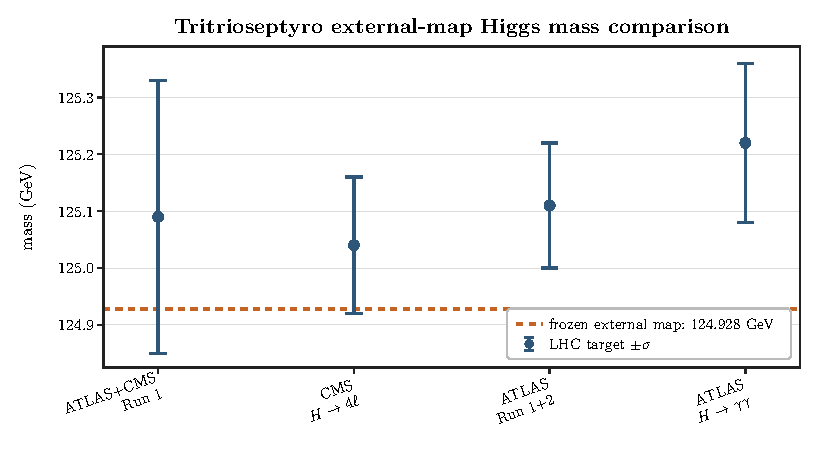
\includegraphics[width=0.92\linewidth,height=0.78\textheight,keepaspectratio]{figures/generated/higgs-mass-comparison.pdf}
\caption{Tritrioseptyro mass comparison. The frozen external map $E_H=RD\,2^{L+4}$ MeV sends the selected candidate to $124.928\,\mathrm{GeV}$. Target records enter as declared external comparison rows.}
\label{fig:manual-higgs-mass-comparison}
\end{figure}

\paragraph{Falsification and external data-comparison record.}
The four target rows overlap in experiment, run, or channel, so their pulls are not four
independent tests; a joint test requires shared covariance and explicit model/map
uncertainty. The internal trace selects $K^{\star}_H=3:3:7_{\mathrm{yro}}$ with
frozen map

\[
E_H^{(0)}=RD_H2^{L+4}=61\cdot2^{11}\,\mathrm{MeV}=124.928\,\mathrm{GeV}.
\]

Table~\ref{tab:manual-higgs-lhc-comparison} records the declared Higgs mass-input rows, their quoted uncertainties, and the resulting $\Delta E$, $|\epsilon|$, and $z_{\mathrm{target}}$ coordinates. The mapped value $124.928\,\mathrm{GeV}$ lies within $1\sigma$ of the ATLAS+CMS Run-1 combined mass record and the CMS Run-2 $H\to4\ell$ mass record while remaining a target-only diagnostic. Production-channel and decay-channel residual tables carry the next comparison layer.

\aodprovenance{\mainsection{main:subsec:yro-odd-window-route-status}; \mainappendix{main:app:ao-field-fractal-properties}; \tabref{tab:manual-higgs-internal-candidates}; \tabref{tab:manual-higgs-external-map}.}

\aodliteraturenote{ATLAS+CMS Run-1 combined mass~\cite{atlas-cms-higgs-run1}. CMS $H\to4\ell$ mass~\cite{cms-hig-21-019}. ATLAS combined Run-1+Run-2 mass~\cite{atlas-higgs-mass-combined-2023}. ATLAS diphoton mass~\cite{atlas-higgs-diphoton-2023}.}
